After collecting the data, I can take the average value of $f_0 = \SI{196.22}{Hz}$ as the constant value of $f_0$ for Equation (\ref{eqn39}). Now I can plot the graph relating $\Delta f$ and $l_n$. The range of the graph corresponds with the distance between the nut and the highest fret of the guitar to the bridge, where the fretboard is. My guitar has 22 frets, so the position of the final fret is
\begin{align*}
    l_{22} = \frac{.648}{2^{\frac{22}{12}}} = \SI{0.182}{m}
\end{align*} 
Therefore the range I will be graphing is $\{0.182 \le l_n \le 0.648 \}$. Below is the general form of the graph.\par
\FloatBarrier
\begin{figure}[!ht]
    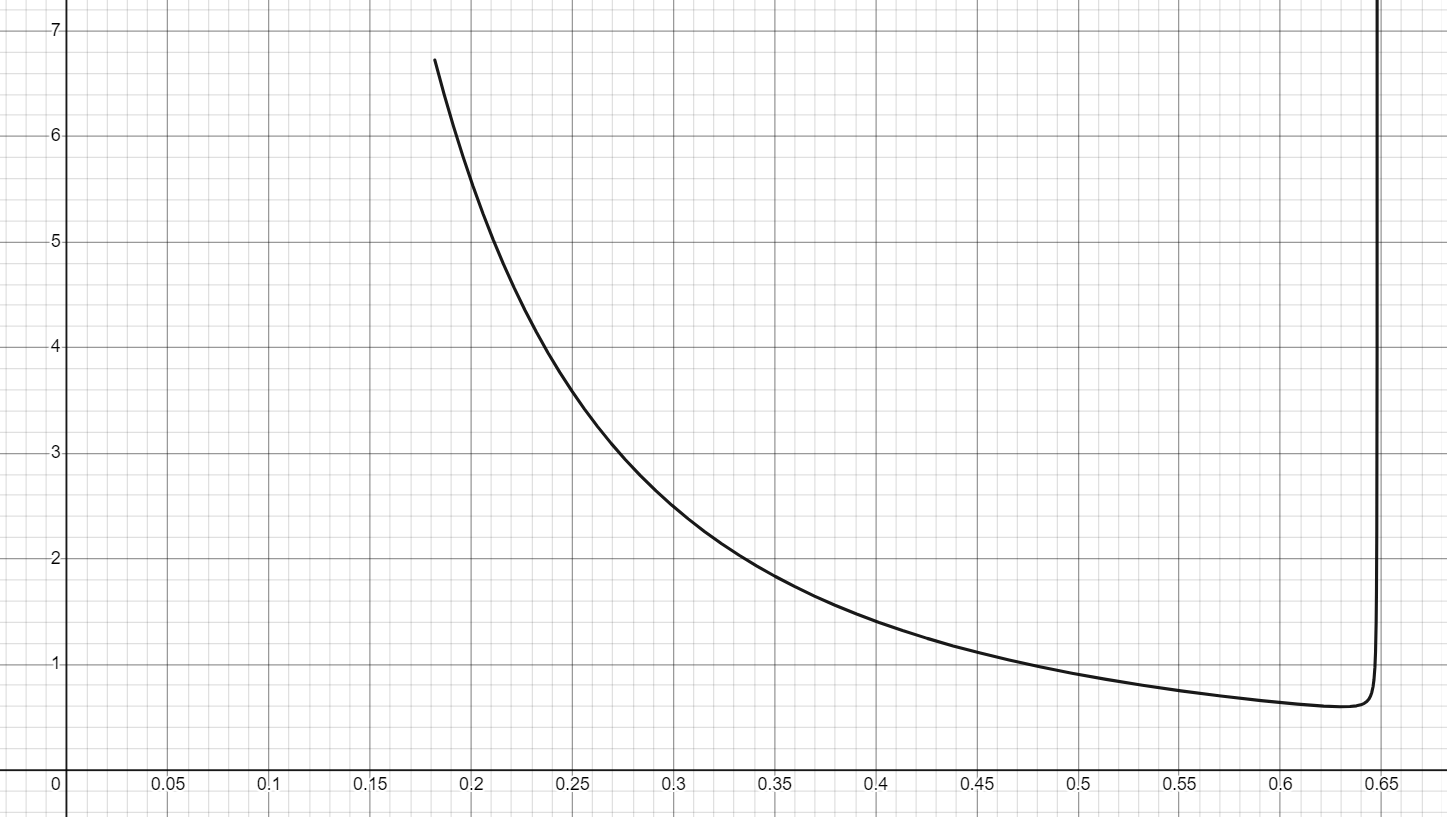
\includegraphics[width = \textwidth]{./ee/no_data_graph.png}
    \caption{General form of the graph without data points} \label{fig7}
\end{figure}
\FloatBarrier
From the graph, we can see it matches with my expectation. Overall $\Delta f$ is lower for larger $l_n$ (further from the bridge, lower frets), and increases when $l_n$ is smaller (higher frets, closer to the bridge). A noticeable thing is the function has no zero in this range, meaning everywhere you fret on the fretboard there will still be a bit of intonation error making it impossible to achieve perfect intonation.\par
Observing the graph, we can see there is a vertical asymptote at $l_n = l$. Mathematically this comes from equation ($\ref{eqn39}$) when the denominator of the terms inside brackets is equal to 0 ($l-l_n = 0$) (there is another asymptote at $l=0$, but this is outside our range). At $\lim_{l_n \to l^-}$ $\Delta f$ approaches $+\infty$. This is physically impossible. My explanation of this is because of the error terms in our first order approximation. When $l_n \approx l$ (very close to the nut), $l-l_n$ is very small and on a comparable order to the nut height $b$, the approximation at (\ref{eqn24}) no longer holds because the higher order error terms will take over. This means the function will no longer accurately model the behavior of the string at that point. My physical interpretation of this phenomenon $\Delta f \to +\infty $ is because, if you try to fret very close to the nut, the "breaking angle" (angle between the fret and the string) $\theta$ of the string in Figure \ref{fig8} gets very large. Therefore, the amount of force downwards needed to counteract the tension to depress the string to touch the fret is much higher, which also increases the tension of the string accordingly, which then in turn requires an even larger force to fret down, increasing the tension even more, etc. This behavior of the tension causes the frequency to rise asymptotically the closer you get to the nut. This will continue until the tension in the string is too large and the string breaks. However, this doesn't happen in reality because the first fret is at $l_n = 0.612$, and you cannot fret closer to the nut than this (albeit for fretless instruments you can go as close as physically possible until the string breaks). \par
\begin{figure}[!htb]
    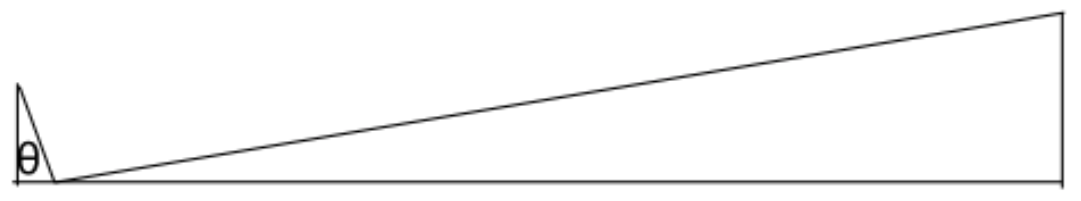
\includegraphics[width=\textwidth]{./ee/breaking_angles.png}
    \caption{Breaking angle $\theta$ of string when fretting near the nut} \label{fig8}
\end{figure}
To analyze the graph further I can take the first derivative of this with respect to $l_n$. The first derivative has a zero at $l_n = 0.625$ m, and substituting this back into the original function we get $\Delta f = 0.087$ Hz. This is a minimum on the graph, indicating that at this point there is the least intonation error. The closest fret to this is fret 1, at $l_n = 0.612$ m. This shows that on the whole fretboard, the intonation error is the smallest at fret 1, and increases as you go higher up the fretboard. The local maximum is at the last fret, fret 22 at $l_n = 0.182 $m. Here the $\Delta f$ is 4.96 Hz, which is a relatively large intonation error.

Also from the graph, the predicted $\Delta f$ at fret 12 ($l_n = 0.324$m) is $\SI{1.15}{Hz}$. This deviation can be put in terms of cents, which is defined as the difference between the frequencies of two consecutive notes divided into 100 equal parts \cite{cents}. Therefore:
\begin{align*}
    \text{1 cent above D4} &= \frac{\text{D\#4 - D4}}{100} \\  
    &= \frac{311.33-293.66}{100} = \SI{0.177}{Hz} 
\end{align*}
(Note values taken from \cite{freq_chart}) \\
So 1.15 Hz is equivalent to $\frac{1.15}{0.177} \approx $ 6-7 cents sharp. The smallest difference in pitch human can discern is around 5-6 cents \cite{loeffler}, and this possibly explains why the intonation error gets noticeable from fret 12 and upwards. \par
Now I can plot a graph with the data points and perform a goodness-of-fit test to determine the correlation.
\begin{figure}[!h]
    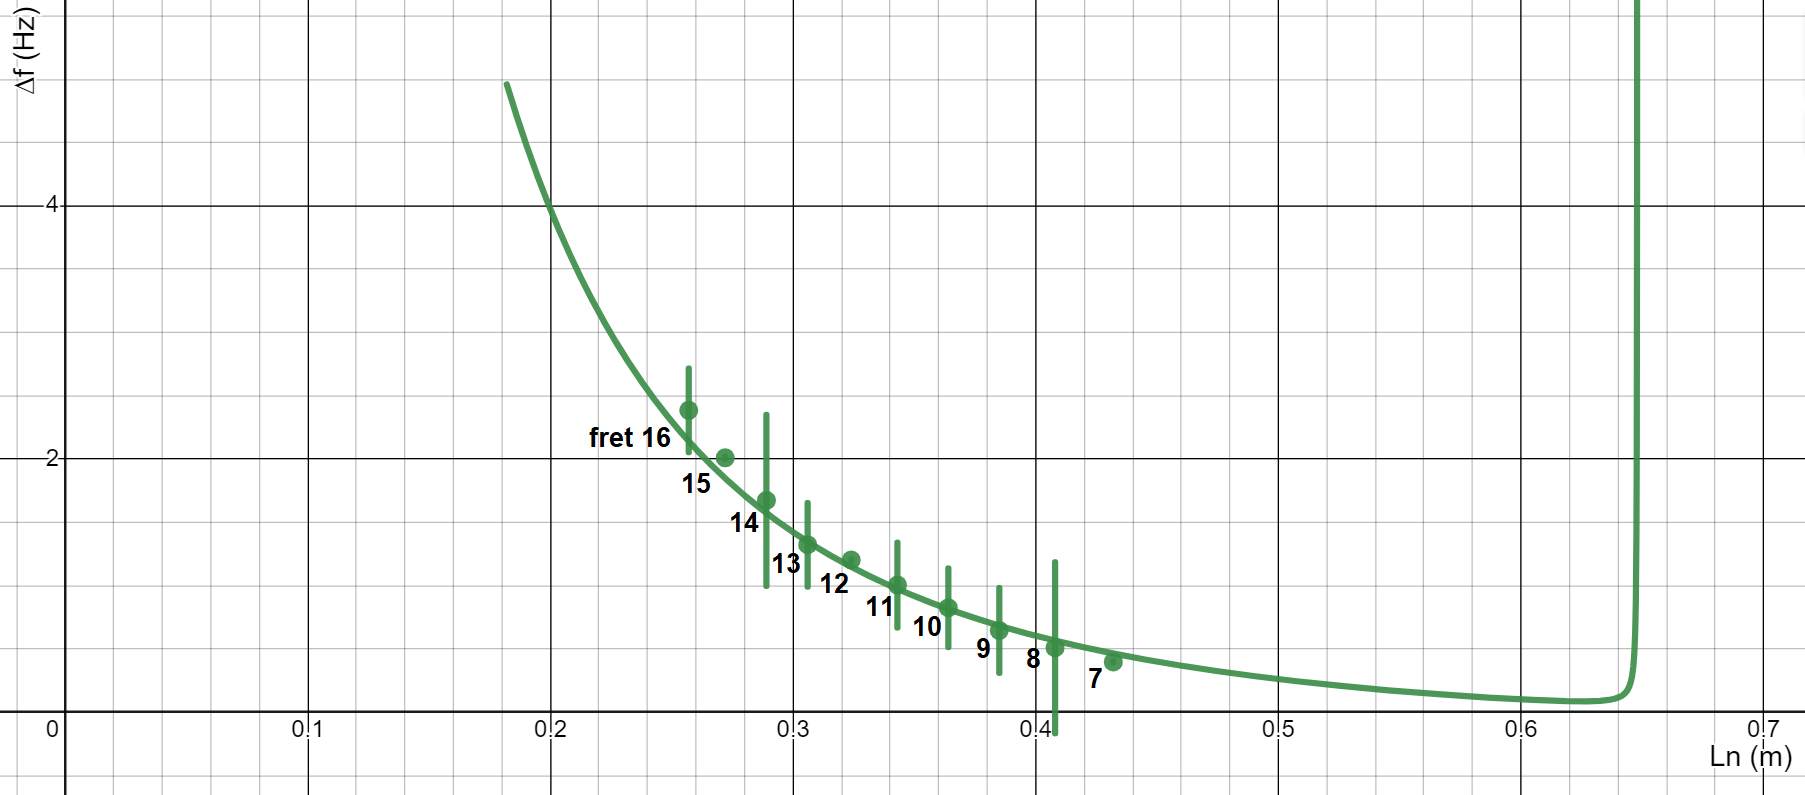
\includegraphics[width = \textwidth]{./ee/graph_with_data.png}
    \caption{The original curve and the data points with error bars} \label{fig9}
\end{figure}